\documentclass[11pt, fullpage,letterpaper]{article}

\usepackage[margin=1in]{geometry}
\usepackage{url}
\usepackage{amsmath}
\usepackage{amssymb}
\usepackage{xspace}
\usepackage{graphicx}
\usepackage{hyperref}
\usepackage{listings}
\usepackage{bm}
\usepackage{float}
\usepackage{graphicx,color,epsfig,rotating}
%\usepackage[demo]{graphicx}
\usepackage{subcaption}


\newcommand{\semester}{Spring 2019}
\newcommand{\myname}{Xiang Zhang}
\newcommand{\myid}{u1199149}
\newcommand{\tbf}{\textbf}


\newcommand{\bx}{{\bf x}}
\newcommand{\bw}{{\bf w}}


\title{A Convergence Study of the Federated Learning Problem with Dynamic Global Update Interval Scheduling and Data Shuffling}
\author{Nicholas Woolsey, Xiang Zhang\\ \{nicholas.woolsey, xiang.zhang\}$@$ utah.edu}

\begin{document} %% begin doc
\maketitle
\begin{enumerate}
\item \tbf{Link to Github page}

All of the ML simulations and implementations can be found at \\ \url{https://github.com/nwoolsey/MachineLearningSpring2019/tree/master/CourseProject} and \url{https://github.com/xiangzhang-122/Machine_Learning/tree/master/CourseProject}. Unfortunately, due to the amount of work to be presented, we were not able to fold all the results into only six pages.

\item \tbf{Problem Formulation \& Motivation}\\
\begin{figure}
  \centering
  \includegraphics[width=0.6\linewidth]{sys_architecture}
\caption{The federated learning framework.}
\label{fig_archt}
\end{figure}
We consider the federated learning framework (also referred to as distributed gradient descent (DGD), or distributed learning. See Figure \ref{fig_archt}) where a set of distributed workers $\{1,2,\cdots, N\}$ works collectively to learn a model from a large dataset $\mathcal{D}$ which consists of $N$ non-overlapping subsets $\mathcal{D}_1, \mathcal{D}_2, \cdots, \mathcal{D}_N$, i.e., $\mathcal{D} = \cup_{i=1}^N\mathcal{D}_i$. Dataset $\mathcal{D}_i$ is only available to worker $i$ and is referred to as the worker's \emph{local dataset}. The learning process is composed of \emph{local updates} and \emph{global aggregation} (or \emph{global update}). Each local update corresponds to one iteration of the model parameter update based on worker $i$'s local dataset $\mathcal{D}_i$. This updating can either be full gradient descent or SGD. After every $\tau$ local updates, the master node which is responsible for aggregating the individually updated weights from all the workers, communicates with the workers and collects these individual weights, doing an averaging of the collected weights \cite{ref4} and then sending the weighted average back to the workers as their initial model parameter to begin a new round of local update.

Assume that global aggregation (or global update) is performed every $\tau$ local updates and in total $T$ global aggregations are performed. For a model parameter $\bw$, we denote $F(\bw)$ as the loss on the whole dataset $\mathcal{D}$ and $F_i(\bw), i=1,2,\cdots,N$ as the loss on local dataset $\mathcal{D}_i$. That is,
\begin{eqnarray}
{\rm Individual \;loss:\;}F_i(\bw)&\triangleq& \frac{1}{|\mathcal{D}_i|}\sum_{j\in \mathcal{D}_i}f_j(\bw)\\
{\rm Overall\;loss:\;}F(\bw)&\triangleq &\frac{\sum_{j\in \cup_{i=1}^{N}|\mathcal{D}_i|F_i(\bw)}}{|\cup_{i=1}^{N}\mathcal{D}_i|}=\frac{\sum_{j\in \cup_{i=1}^{N}D_iF_i(\bw)}}{D}
\end{eqnarray}
where $f_j\triangleq f(\bw, \bx_j,y_j)$ is the loss evaluated at one data point $(\bx_j,y_j)$ and $D_i=|\mathcal{D}_i|,D=\sum_{i=1}^ND_i$. Our goal is to minimize the overall loss function by finding the optimal weight $\bw*$ regarding the whole dataset $\mathcal{D}$. More specifically, let $\bw_i(t)$ denote the locally updated weight by worker $i$ at the $t$-th iteration, and we define $\bw(t)\triangleq \frac{\sum_{i=1}^ND_i\bw_i(t)}{D}$. The local update of worker $i$ is then
\begin{eqnarray}
\bw_i(t) = \tilde{\bw}_i(t-1)-\gamma(t) \tilde{\bw}_i(t-1)
\end{eqnarray}
in which $\gamma(t)$ is the variable stepsize scheduling function defined as $\gamma(t)\triangleq\frac{\gamma_0}{1+\frac{\gamma_0}{d}t}$ with parameters $\gamma_0$ and $d$ to be tuned to accelerate convergence. $\tilde{\bw}_i(t-1)$ represents the initial values of the weight at the beginning of the $t$-th iteration. Depending on whether a global update  is performed or not at the end of the $(t-1)$-th iteration, $\tilde{\bw}_i(t-1)$ can take different values. More specifically, is the global is performed, then $\tilde{\bw}_i(t-1) = \bw(t-1)=\frac{\sum_{i=1}^ND_i\bw_i(t-1)}{D}$. Otherwise, we have $\tilde{\bw}_i(t-1) = \bw_i(t-1)$.

We consider a computation resource constrained distributed learning system where the each local update at a single worker consumes $c$ units of resource and each global update consumes $b$ units of resource. As stated before, the total number of iterations performed by each worker is equal to $K\triangleq  T\tau$. Hence, the final output of the aggregator is $\bw(K)=\frac{\sum_{i=1}^ND_i\bw_i(K)}{D}$ implying that global update is always performed at the end of the iterations. The total resource consumed by the workers is equal to $C_{\rm worker}=NT\tau c=NKc$ units and the total resource consumed by the aggregator is equal to $C_{\rm aggregator} = Tb$ units. Assume a total resource budget $R$, our goal becomes
\begin{eqnarray}
\min_{K, \tau} & \;& F(\bw(K))\\
{\rm s.\;t.} &\;& C_{\rm worker} +C_{\rm aggregator}= K\left(Nc +\frac{b}{\tau}   \right) \le R
\end{eqnarray}


\item \tbf{Project Ideas \& Methodology}

The paper \cite{ref4} focus on achieving the overall loss function minimization goal by setting $\tau$ to stay unchanged during the entire the iterating process. We have several important observations which leads to the ideas of this project. We empirically justified our ideas by using both artificially generated data and the real-world data. These observations and ideas are list below.
\begin{enumerate}
\item \tbf{Dynamic Scheduling of Global Updating Intervals (GUI)\footnote{Global updating interval refers to the number of local updates performed by each worker between two consecutive global updates.}} One important observation is that when $\tau =1$, the distributed gradient descent is equivalent to the centralized full gradient descent algorithm due to the linearity of the the gradient operator. This observation leads to our project idea of considering a time-varying $\tau=\tau (t)$, which provides more flexibility in controlling the convergence process. More specifically, let us define \emph{individual minima}, denoted by $\bw_i^*(\mathcal{D}_i)$ as the optimal weight that minimizes the local loss $F_i(\bw)$. We also denote the \emph{global minima} $\bw^*$ as the optimal weight that minimizes the overall loss function $F(\bw)$. Each local update leads the local weight $\bw_i(t)$ closer to the individual minima $\bw_i^*(\mathcal{D}_i)$. The role of global updating is to find the average of all the individual minima (denoted by $\bw_{\rm avergae}\triangleq \frac{D_i\bw_i^*(\mathcal{D}_i)}{D}$) and pulls the averaged weight closer to the global minima $\bw^*$. An extreme case is that when $\tau =1$, the DGD becomes the centralized full gradient descent algorithm. However, as we have found empirically, the average of the local minima does not necessarily equal the global minima. Based on this, we can have a clearer understanding of the effect of large and small values of $\tau$. Under a given resource budget $R$, on one hand, if $\tau$ is large, meaning that global aggregation is less frequently performed, the individual weights are converged more to their individual minima and the final output approaches the average of these individual minima which is not necessarily equal to the global minima $\bw^*$ desired. On the other hand, if $\tau$ is small, meaning that global updates are performed more frequently, the averaged weights are constantly pulled toward the global minima $\bw^*$ due to the effect of averaging. Two extreme cases are $\tau=K$ and $\tau=1$. When $\tau = K$, only one global update is performed at the end of the process, the output $\bw(t)$ stops exactly at the average of the these individual minima. When $\tau = 1$, the process is 'synchronized' to the centralized gradient descent at each step of iterations, and the final output is the global minima $\bw^*$, which is also the output of the centralized GD algorithm. However, small values of $\tau$ imposes a heavy communication load between the global aggregator and workers, implying a tredeoff between communication and convergence accuracy. For the values of $\tau$ in between, i.e., $1<\tau <K$, there is compromise of the two extreme effects: global updating pulls the updated weight to the centralized global minima $\bw^*$ and each epoch of the local updates leads the individual weight closer to their individual minima $\bw_i^*$, thus pulling the averaged weight towards $\bw_{\rm average}$. The result can be easily imagined to be some bouncing between $\bw^*$ and $\bw_{\rm average}$ as the number of iterations increases (we visualized this bouncing effect later in this report). Since we empirically found that $\bw^*\neq \bw_{\rm average}$, fixing $\tau$ to be a constant greater than 1 is not a good idea in the sense that the expectation of the output weight of the federated learning algorithm is not equal to the global minima weight of the overall loss function, minimizing which should be our ultimate pursuit.

Based on this observation, we propose the concept of \emph{dynamic scheduling of $\tau =\tau(t)$}, where $\tau(t)$ varies along the number of iterations increases. The idea is easy to understand but efficient. Given a resource budget $R$, the total number of local and global updates is literally determined. We simply assign larger values to $\tau(t)$ is the iteration index $t$ is small and as $t$ increases, we assign smaller values to $\tau(t)$ such that the global updates is performed more frequently ans the averaged weight is  puller towards the global minima $\bw^*$. We assign values to the decreasing series $\{\tau(t)\}_{t=0,1,2,\cdots,K}$ such that the resource budget $R$ is satisfied. Moreover, since at the beginning the workers communicate less frequently with the aggregator and more frequently when the updating process proceeds, it is possible to satisfy the communication constraint by designing $\{\tau(t)\}_{t=0,1,2,\cdots,K}$. As a result, we can formulate a new problem as
\begin{eqnarray}
\min_{K, T, \{\tau(t)\}_{t=0,1,2,\cdots,K}} & \;& F(\bw(K))\\
{\rm s.\;t.} &\;& C_{\rm worker} +C_{\rm aggregator}= \sum_{i=1}^TN\tau'(i)c+Tb \le R\\
&\;&  \sum_{i=1}^{T}\tau'(i) =K
\end{eqnarray}
in which $\tau'(i), i=1,2,\cdots,T$ denotes the global update interval between the $i$-th and $i+1$-th global updates. There are multiple scheduling strategies for the GUI. For example, we can use exponential decay, i.e., after every certain number of iterations, reduce the GUI $\tau$ by half until it reaches 1, which guarantees that the DGD algorithm converges to the global minina $\bw^*$. We empirically showed the effectiveness of the exponential decay scheduling later in the report using the linear regression model.
\item \tbf{The Effect of Data Shuffling\footnote{Data shuffling here refers to the exchange of the data points among different workers instead of shuffling the order of passing through a fixed dataset by the SGD algorithm.} among Workers} In the federated learning/DGD setting, each worker $i$ only has access to a $|\mathcal{D}_i|/|\mathcal{D}|$ portion of the whole dataset $\mathcal{D}$  on which the loss function needs to be minimized. intuitively, data shuffling can help in the sense that each worker sees more data and thus facilitates better convergence after aggregation. We first proposed a baseline shuffling scheme called \emph{naive data shuffling} in which at the beginning of each new round of local updates, a certain fraction (determined by the \emph{shuffling parameter $\alpha$}, defined as the fraction of exchanged for each of the local dataset $\mathcal{D}_i$) of the local data of a worker $i$ is replaced by the data points from other workers' local datasets chosen at random. Unfortunately, naive data shuffling does not help much to the convergence and in some cases the convergence speed is even a bit worse. As shown later in Section 6, constantly shuffling the data after each global update is not a good idea since it changes the optimal weight $\bw_i^*$ of each local dataset $\mathcal{D}_i$ constantly, leading the averaged weights to some  oscillations. More specifically, in each local updating epoch, worker $i$ starts with the globally updated weight as the initial weight, and each local update leads the weight $\bw_i(t)$ one step closer to its local optima $\bw_i^*$ (if we assume convecity of the loss function). However, if we shuffle these local datasets, then each worker $i$ will see a different portion of data, $\mathcal{D}_i'$, and the following local updates of worker $i$ will head toward a new local optima $\bw_i^{*}$ $'$ over the new local dataset $\mathcal{D}_i'$. Since the set of local optima changes, the averaged weights changes according to the distribution of the new set of local optima. Depending on the specific set of data $\{\mathcal{D}_i\}_{i\in[N]}, \cup_{i\in [N]}\mathcal{D}_i =\mathcal{D}$ the workers have, the set of local optima $\{\bw_i^*\}_{i\in [N]}$ is different from each other. Each realization of data shuffling corresponds to a new set of  local optima, and the average of which can be either far or close to the global optima $\bw^*$. Doing random shuffling does not give any guarantee on the closeness of the averaged weight to the global optima. Hence, there should be some way to design smarter data shuffling scheme such that the averaged weight is guaranteed to be close enough to the global optima $\bw^*$. Due to the limited time, we are not able to find the proper shuffling schemes with guarantee of closeness (or convergence). However, we will still work on this problem as a research direction and try to figure out if coding of data can help to improve convergence.



\end{enumerate}

\item Midterm Initial Result Review

In this section we briefly review the initial results we obtained in the mid-term result. In our first experiment, we aim to observe the impact to distributed ML when nodes have a varying amount of noise in their respective data set. In general, the perceptron algorithm is performed under $3$ scenarios. First, we assume all of the data is collected at a single node (or in the cloud) and processed. Next, we consider the distributed case where $n$ nodes perform local epoch updates. After every $\tau$ updates, the nodes perform a global update where the learned weights of each node are sent to a central node. We consider two types of global updates, such that either the mean or the median of the collected weights is computed. The computed global weights are pushed back to the nodes which start training again using the globally updated weights to start.

The exact setup to this experiment is as follows. An absolute weight vector is arbitrarily generated to be $w^* = [1,1,1,1,1,1,1,0]$ (includes bias term). Then, $nP$ examples on $\mathbb{R}^7$ are generated using a $(-1,1)$-uniform distribution for each dimension, where $P$ is the number of examples at each node. Moreover, $n=8$ and $P=200$. True labels are computed for each example using the absolute weights. Noise is then added to the data. We defined a noise vector $N=[0.1, 0.1, 0.1, 0.1, 0.1, 0.1, 10, 10]$ which defines the power of the Gaussian noise added to the examples. The noise is heterogeneous in that, $2$ of the noise have much more noisy data than the other $6$ nodes.

Then training is performed by the $3$ methods discussed above, and for each case the learning rate is set to $r=0.0001$. For each method, the training has $T=100$ global iterations, where in each global iteration, $\tau=10$ epochs are performed. For the centralized case, basically $1000$ epochs are performed by the traditional perceptron algorithm. Alteratively, each node performs $\tau$ epochs on its local data, then the weights are globally updated using either the mean or median function and this is considered a $1$ global iteration. After each global iteration (or simply $\tau$ epochs for the centralized case), a set of test data without noise is used to determine the test error rate. The results are shown in the following figure.

\par{\hspace*{1cm}\includegraphics[width=12cm]{Figure_0.png}}

Performing this experiment not only provided a base Python code for future experiments, but these initial results give some interesting insight into future directions of this project. First, it is clear that the centralized method trains fast than the decentralized ones. In this simple example we only studied the two extreme cases of completely centralized or decentralized, it may be interesting in future experiments to see how ``overlapping" data sets affects the speed of training or how nodes shuffling data (to simulate overlapping data sets) could improve the speed of training.

Another interesting observation is that the decentralized mean and the centralized perceptron methods converge to the same test error. This matches previous findings in literature that claim these two methods should converge similarly. Of course, those results were based on a homogeneous setting, so it is interesting to see that in the heterogeneous setting that the same observation occurs.

Finally, it is clear that after enough training, the decentralized perceptron method with median aggregation outperforms the other methods. This surprising result demonstrates that there may be an advantage to distributed ML in a heterogeneous setting and gives further motivation to study this topic. While effectively, it is unknown which nodes have noisy data, the median global aggregation acts to cancel the effects of the noisy data. Ultimately, it will be interesting to see if data shuffling can speed up ML, but clearly these results demonstrate that there might be some benefit to labeling the data with its origin.


\item Effect of Naive Data Shuffling

In this section we present the simulation results about the effect of naive data shuffling on soft SVM, where after each global update, a fraction of the local datasets owned by two workers are randomly exchanged. The simulation results is based on two datasets, one is the artificial dataset with 300 samples\footnote{Refer to the Linear regression section for the detailed data generating process} and the other is the real-world UCI banknote dataset containing 872 samples which we used many times in the homework.

The experiment setup is as follows: We implement the soft SVM on a federated learning system with $N=2$ workers each having half of the entire dataset. For local updates, SGD is used to pass through the local dataset $\tau$ times between any two global updates. The order of passing the local data set is randomly changed after each every passing of the local dataset. A simple data shuffling scheme is employed. We defined the \emph{shuffling parameter $p\in[0,1)$} as the fraction of exchanged data for each worker after data shuffling, which is a measure of the amount of new samples seen by a worker. More specifically, denote the two local datasets of the two workers as $\mathcal{D}_1$ and $\mathcal{D}_2$ which are assumed to have equal size, i.e., $|\mathcal{D}_1|=|\mathcal{D}_2| $. We randomly select $\lfloor p|\mathcal{D}_1|\rfloor$ samples $\mathcal{S}_1$ from $\mathcal{D}_1$ and select $\lfloor p|\mathcal{D}_2|\rfloor$ samples $\mathcal{S}_2$ from $\mathcal{D}_2$ and exchange them between without replacement between the two workers, that is, the new local datasets after data shuffling is $\mathcal{D}_1'=(\mathcal{D}_1\backslash \mathcal{S}_1) \cup \mathcal{S}_2$ and $\mathcal{D}_2'=(\mathcal{D}_2\backslash \mathcal{S}_2) \cup \mathcal{S}_1$. The convergence results are shown in the following.

\begin{figure}
\centering
\begin{subfigure}{.5\textwidth}
  \centering
  \includegraphics[width=\linewidth]{figure_1}
  \caption{Shuffling parameter setup 1, $\tau =1, T=100$}
  \label{fig_11}
\end{subfigure}%
\begin{subfigure}{.5\textwidth}
  \centering
  \includegraphics[width=\linewidth]{figure_2}
%  \caption{$T=2$}
 \caption{Shuffling parameter setup 2, $\tau =1, T=100$}
 \label{fig_12}
\end{subfigure}
\begin{subfigure}{.5\textwidth}
  \centering
  \includegraphics[width=\linewidth]{figure_3_tao2}
  \caption{Shuffling parameter setup 3, $\tau =2, T=100$}
  \label{fig_13}
\end{subfigure}%
\begin{subfigure}{.5\textwidth}
  \centering
  \includegraphics[width=\linewidth]{figure_4_tao2}
%  \caption{$T=2$}
 \caption{Shuffling parameter setup 4, $\tau =2, T=100$}
 \label{fig_14}
\end{subfigure}
\caption{Convergence speed comparison based on the artificial dataset.}
\label{fig_1}
\end{figure}

Fig. \ref{fig_1} shows the convergence (loss function values versus the number of global updates) result for various shuffling parameter $p$ values on the artificial dataset with $\tau =1$. From Fig. \ref{fig_11} we see that shuffling with $p=0.6,0.9$ achieves slightly better convergence than no shuffling, and $p=0.1$ has similar convergence as no shuffling. $p=0.4$ achieves a worse convergence speed than no shuffling. We observed similar effects in Fig. \ref{fig_12}. This result reveals that naive shuffling does not always help to increase the convergence speed and if it helps, the effect is very limited compared to the centralized convergence curve (Fig. \ref{fig_14}). This result is somehow counter-intuitive. At least for now, we need to think more about how to employ data shuffling schemes to improve convergence given the evidence that a naive random shuffling does not always help.
\begin{figure}
  \centering
  \includegraphics[width=0.6\linewidth]{fig_no_shuffle}
\caption{Convergence speed comparison based on the artificial dataset.}
\label{fig_3}
\end{figure}

Fig. \ref{fig_3} shows the convergence speed for multiple different values of $\tau\in\{1,2,6,16,32\}$ and $T=100$. It can be seen that there is a limited convergence speed improvement as we increase $\tau$, which can interpreted as: as the SGD pass through the local dataset more and more between two global updates, the 'useful information' contained in that local dataset are fully exploited so increasing $\tau$ does not help to improve convergence anymore. The effect may imply that data shuffling is indeed necessary to let each worker see more data samples in the weight updating process.

Fig. \ref{fig_4} shows the convergence curve on the UCI dataset. In this case, we see that shuffling with parameters $p=0.1,0.5 $ have similar convergence speed which is better than no shuffling. However, when compared to the centralized version curve, the improvement brought by shuffling is very limited. As we have seen before, naive shuffling may not always seem to help. We need to design more 'smart' shuffling schemes, for example, the shuffling should stop at some point since when we are approaching the convergence point, shuffling can induce oscillations in iterative weight updating.
\begin{figure}
  \centering
  \includegraphics[width=0.6\linewidth]{ff_2}
\caption{Convergence speed comparison based on the real-world dataset.}
\label{fig_4}
\end{figure}








\item
\tbf{Linear Regression}

To better understand the behavior of distributed learning, we developed a simulation to track the weights and loss function throughout the training. The data consists of artificially generated data of the form
\begin{align}
y_i = 2x_i + 2 + \upsilon_i
\end{align}
where $x_i$ and $\upsilon_i$ is from zero-mean Gaussian distributions with variance $1$ and $N$, respectively. $N$ can be consider the noise power and adjusted between runs. For each learning simulation new random data is generated. An example of the data is shown in the figure below.



  \begin{figure}[ht]
\begin{center}
\advance\leftskip-3cm
\advance\rightskip-3cm
\includegraphics[width=10cm]{Figure_LR_data.eps}
\caption{Example Data Set}
\end{center}\end{figure}

In this 2-dimensional linear model there are only two weights, which was chosen in order to visualize the weights throughout on the training on a 2-D plot. This will be observed in the figures throughout this section.

The generated data is used to form the matrix $A$ such that

\begin{align}
A = \left[ \begin{array}{c c}
           x_1 & 1   \\
           x_2 & 1   \\
           \vdots & \vdots   \\
           x_m & 1
         \end{array} \right]
\end{align}
and the vector $\boldsymbol{y}= [y_1 \; y_2 \cdots y_m]^\intercal$. The optimal weights based on all the data is defined as
\begin{align}
\boldsymbol{w}^* = (A^\intercal A)^{-1} A^\intercal \boldsymbol{y}
\end{align}
which includes one weight and the bias term (or the second weight). Moreover, $A$ and $\boldsymbol{y}$ is split into $n$ parts such that
\begin{align}
A = \left[ \begin{array}{c }
           A_1   \\
           A_2    \\
           \vdots  \\
           A_n
         \end{array} \right], \;\;\;\; \boldsymbol{y} = \left[ \begin{array}{c }
           \boldsymbol{y}_1   \\
           \boldsymbol{y}_2    \\
           \vdots  \\
           \boldsymbol{y}_n
         \end{array} \right]
\end{align}
where $A_i$ is of size $\frac{m}{n}\times 2$ and $\boldsymbol{y}_i$ is of size $\frac{m}{n}\times 1$. This represents an initialize data distribution among $n$ nodes such that node $i$ has access to training data $A_i$, $\boldsymbol{y}_i$. The global minimum of each data set is
\begin{align}
\boldsymbol{w}^*_i = (A_i^\intercal A_i)^{-1} A_i^\intercal \boldsymbol{y}_i
\end{align}
and let $\bar{\boldsymbol{w}}^*$ be the mean weights of the optimal weights from the $n$ data sets
\begin{align}
\bar{\boldsymbol{w}}^* = \frac{1}{n}\sum_{i=1}^{n}\boldsymbol{w}_i^*.
\end{align}
We compare two training methods where in each case the ``full gradient" approach where a node will perform weights updates using all available data points. The first method is the centralized training method representative of a node that has access to the entire training set. In this setting
\begin{align}
\boldsymbol{w}^{(k+1)} = \boldsymbol{w}^{(k)} - 2r(A^\intercal A \boldsymbol{w}^{(k)} - A \boldsymbol{y})
\end{align}
where $r$ is the learning rate and $2(A^\intercal A \boldsymbol{w}^{(k)} - A \boldsymbol{y})$ is the gradient. Similarly, local updates are performed in the distributed method as
\begin{align}
\boldsymbol{w}_i^{(k+1)} = \boldsymbol{w}_i^{(k)} - 2rn(A_i^\intercal A_i \boldsymbol{w}_i^{(k)} - A_i \boldsymbol{y}_i).
\end{align}
In the distributed method, a global update can be performed such that
\begin{align}
\boldsymbol{w}_i^{(k+1)} = \bar{\boldsymbol{w}}^{(k)} - 2rn(A_i^\intercal A_i \boldsymbol\bar{\boldsymbol{w}}^{(k)} - A_i \boldsymbol{y}_i).
\end{align}
where $\bar{\boldsymbol{w}}_i^{(k)} =\frac{1}{n}\sum_{i=1}^{n}\bar{\boldsymbol{w}}_i^{(k)}$. For both the centralized and distributed methods, we compute the loss function as
\begin{align}
L_c^{(k)} = ||A\boldsymbol{w}^{(k)} - \boldsymbol{y}||^2, \;\;\;\; L_d^{(k)} = ||A\boldsymbol\bar{\boldsymbol{w}}^{(k)} - \boldsymbol{y}||^2
\end{align}
respectively. Note that, for both the centralized and decentralized computation of the loss function the entire data set is used.
\begin{enumerate}

  \item \tbf{Behavior of Local versus Global Updates}

  In the following, we perform simulations to understand the effects of the local versus global updates. First, in the following, only local updates are performed.

  \begin{figure}[H]
\begin{center}
\advance\leftskip-3cm
\advance\rightskip-3cm
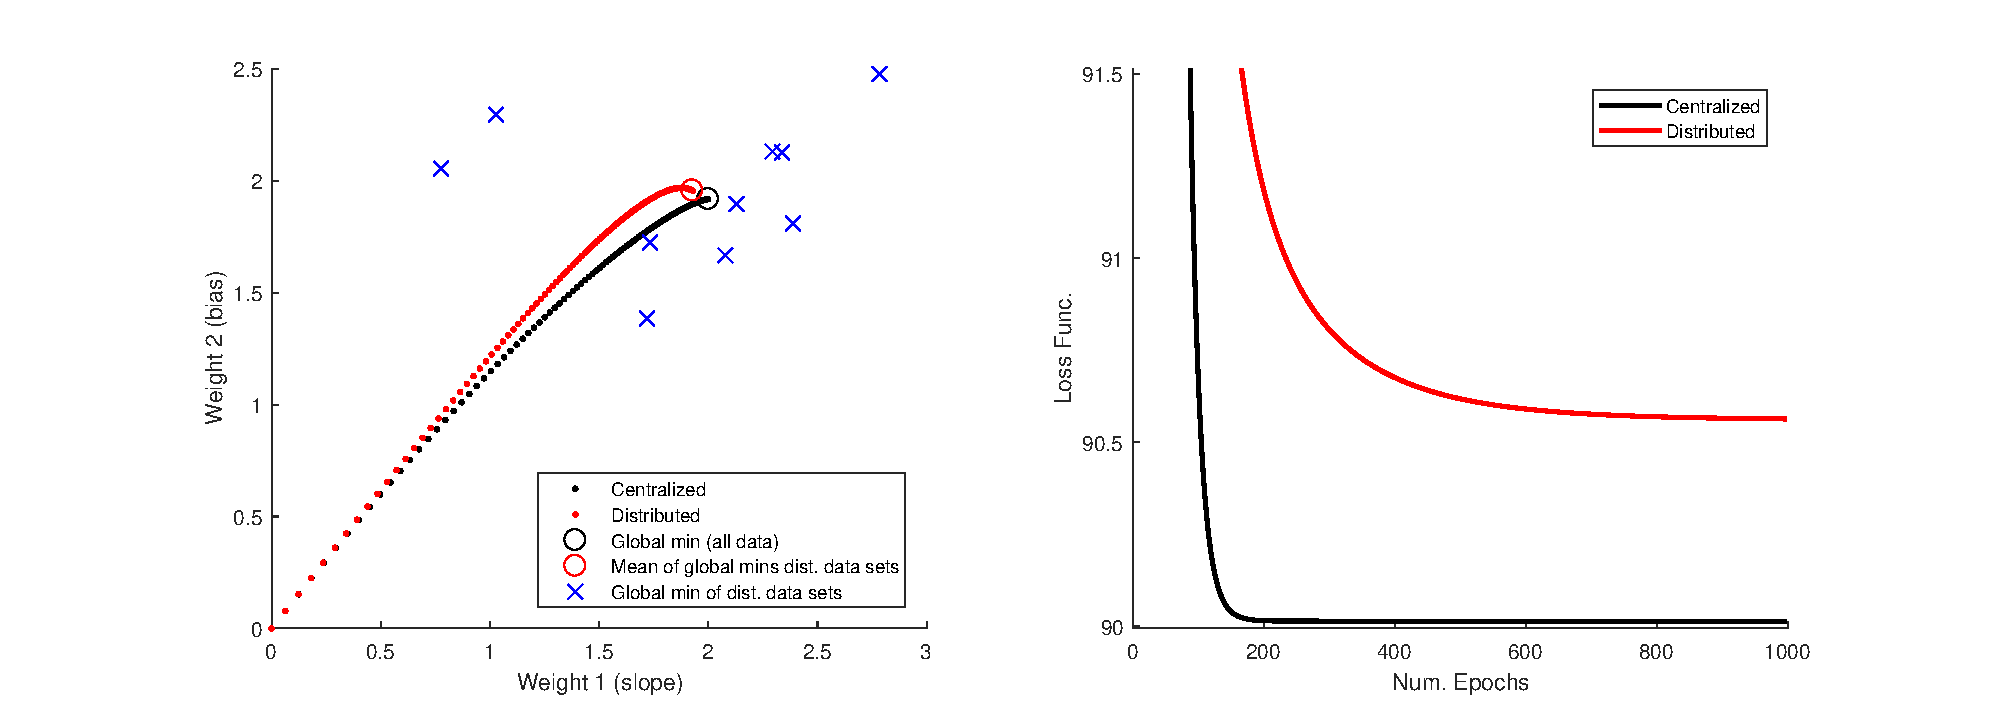
\includegraphics[width=20cm]{LocalUpdates.eps}
\caption{Only Local Updates}
\end{center}\end{figure}

In the above figure, the red dots represent $\bar{\boldsymbol{w}}_i^{(k)}$. Note that, although no global updates are performed. The final result of the distributed learning network will be computed by averaging the results of the nodes. Therefore, we track $\bar{\boldsymbol{w}}_i^{(k)}$ to understand the learning trends of the network. Moreover, the black dots represent the control, centralized learning, where one node has access to all the data. The blue X's represent the global minimums of the distributed data sets. Finally the red circle is  $\bar{\boldsymbol{w}}^*$ and the black circle is $\boldsymbol{w}^*$.

The first important observation is that $\bar{\boldsymbol{w}}^*\neq\boldsymbol{w}^*$. Next, the distributed learning approaches $\bar{\boldsymbol{w}}^*$. This makes sense since each of the nodes is learning approaching the global minimum of their individual data sets. The centralized learning approaches the more optimal $\boldsymbol{w}^*$. While $\bar{\boldsymbol{w}}^*$ and $\boldsymbol{w}^*$ are close, since they are not exactly the same, the two methods converge to different points and therefore have different values of the loss function throughout the training.

Alternatively, we can perform only global updates for the distributed method.

\begin{figure}[H]
\begin{center}
\advance\leftskip-3cm
\advance\rightskip-3cm
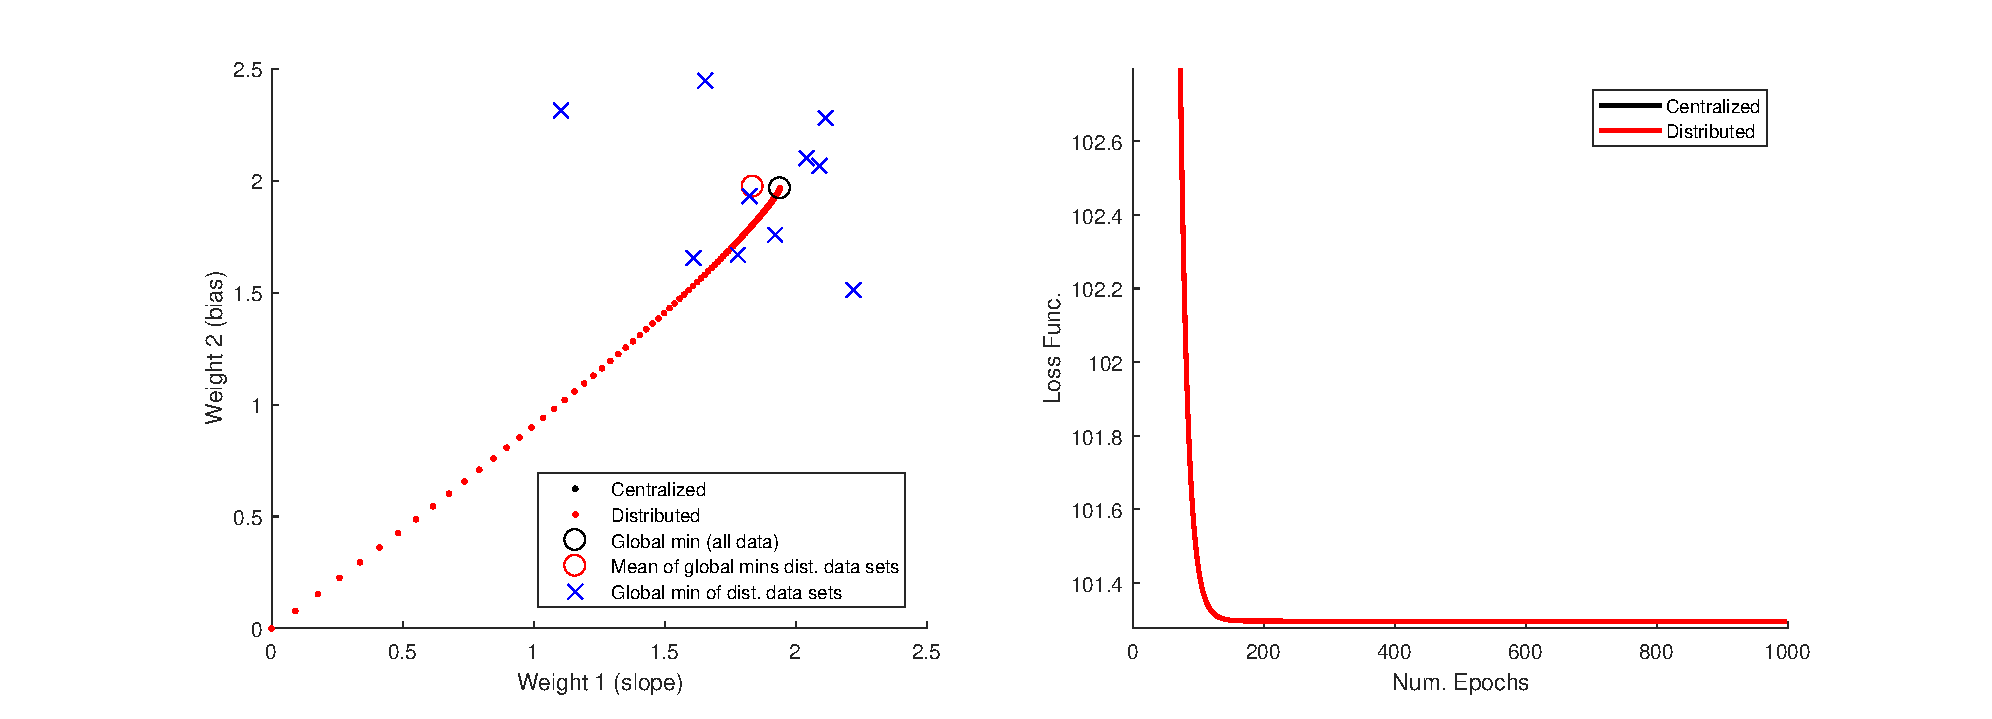
\includegraphics[width=20cm]{GlobalUpdates.eps}
\caption{Only Global Updates}
\end{center}\end{figure}

  In the case both the centralized and distributed methods converge to $\boldsymbol{w}^*$, the optimal weights for the whole data set. In fact, the two methods perform exactly the same in this case. This can be explained observing the global update rule.
  \begin{align}
  \bar{\boldsymbol{w}}^{(k+1)} &= \frac{1}{n}\sum_{i=1}^{N}\boldsymbol{w}_i^{(k+1)} \\
  &= \frac{1}{n}\sum_{i=1}^{N}\left(\bar{\boldsymbol{w}}^{(k)} - 2rn(A_i^\intercal A_i \boldsymbol\bar{\boldsymbol{w}}^{(k)} - A_i \boldsymbol{y}_i)\right)\\
  &= \bar{\boldsymbol{w}}^{(k)} - \frac{1}{n}\cdot 2rn \sum_{i=1}^{N}\left(A_i^\intercal A_i \boldsymbol\bar{\boldsymbol{w}}^{(k)} - A_i \boldsymbol{y}_i\right) \\
  &= \bar{\boldsymbol{w}}^{(k)} - 2r(A^\intercal A \boldsymbol\bar{\boldsymbol{w}}^{(k)} - A \boldsymbol{y})
    \end{align}

  The global update rule for the distributed learning is the same as the update for the centralized learning, therefore, the two methods perform exactly the same.

  \item \tbf{Distributed learning with both local and global updates}

   In \cite{ref4}, the authors discuss the topic of some trade-off between the use of global versus local updates in distributed learning. Moreover, they define a parameter, $\tau$, which defines the number of local updates for every global update. They are motivated by the fact that a global update takes both communication and computation resources and may not be practical to perform many global updates. While the authors gave some theoretical guarantees on the performance based on $\tau$, it is unclear exactly how $\tau$ affects the convergence of the weights. In the following, we study a multiple values of tau and monitor the weights and the loss function throughout training.

   \begin{figure}[H]
\begin{center}
\advance\leftskip-3cm
\advance\rightskip-3cm
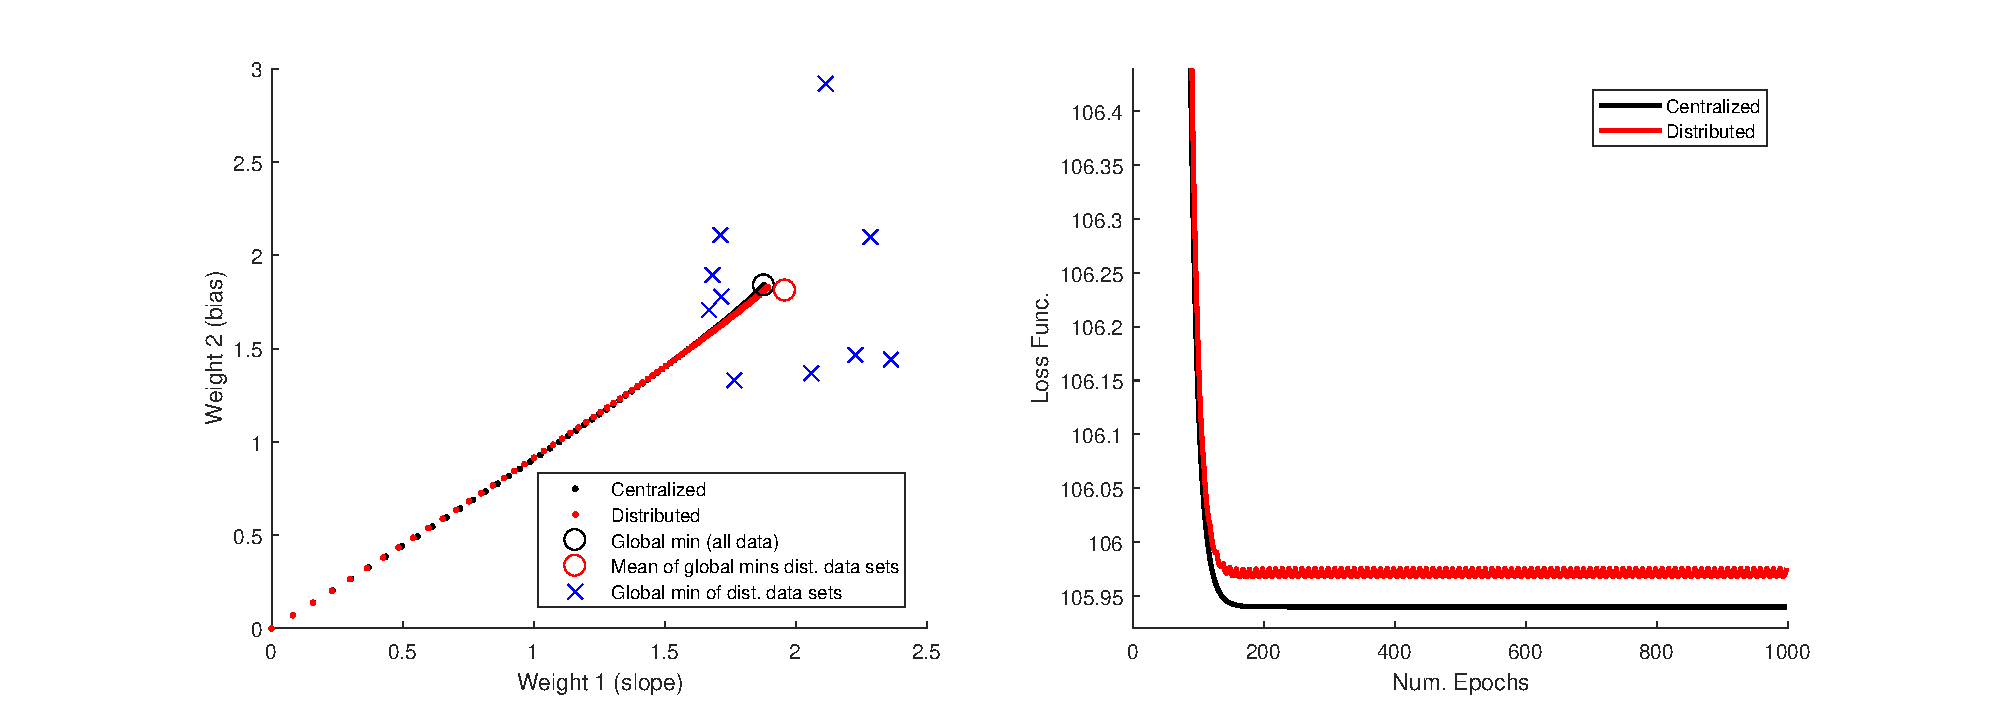
\includegraphics[width=20cm]{tau=10.eps}
\caption{$\tau=10$}
\end{center}\end{figure}

   \begin{figure}[H]
\begin{center}
\advance\leftskip-3cm
\advance\rightskip-3cm
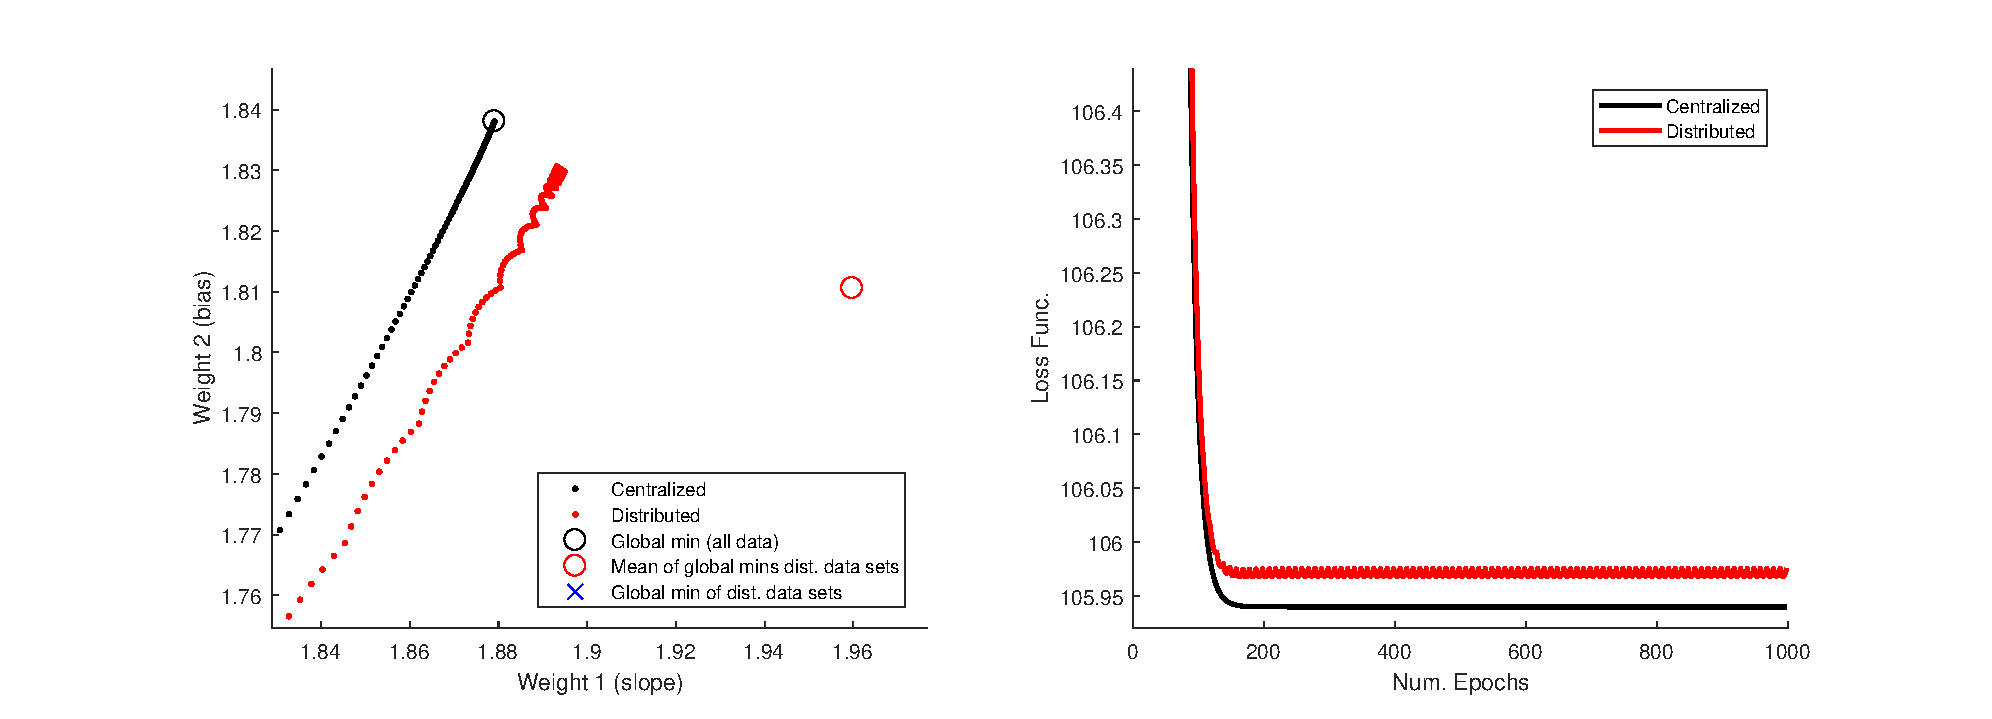
\includegraphics[width=20cm]{tau=10_zoom.eps}
\caption{Zoomed image: $\tau=10$}
\end{center}\end{figure}

We provide two figured for the case where $\tau=10$ which include a zoomed in and zoomed out picture. It appears that the distributed system converges to a point near $\boldsymbol{w}^*$, however, from the zoomed image of the weights and the loss function, we can see it oscillates. This matches some of the previous findings. When a global update is performed, the distributed system begins to converge towards $\boldsymbol{w}^*$, however, as many local updates occur, the weights converge towards $\bar{\boldsymbol{w}}^*$ creating oscillations when using both local and global updates.

Next we observe the cases where $\tau = 100$. Again, two images are provided. The oscillations of the weights and the loss function is more extreme compared to the case where $\tau=10$. This occurs because the nodes perform more local updates are start to get closer to $\bar{\boldsymbol{w}}^*$ as more local updates occur.
   \begin{figure}[H]
\begin{center}
\advance\leftskip-3cm
\advance\rightskip-3cm
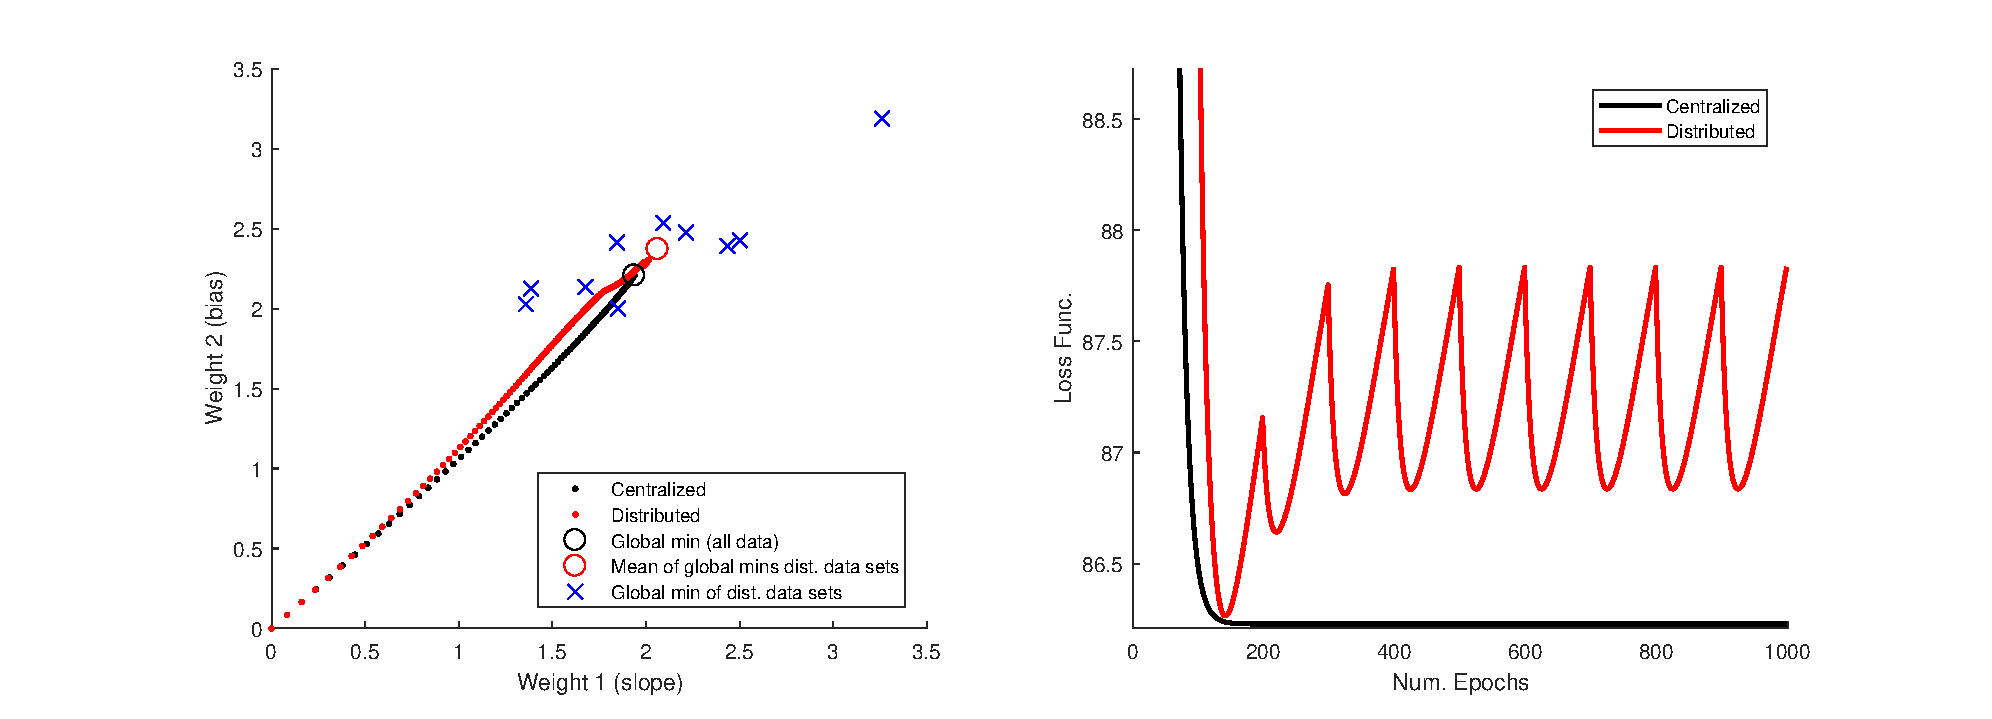
\includegraphics[width=20cm]{tau=100.eps}
\caption{$\tau=100$}
\end{center}\end{figure}

   \begin{figure}[H]
\begin{center}
\advance\leftskip-3cm
\advance\rightskip-3cm
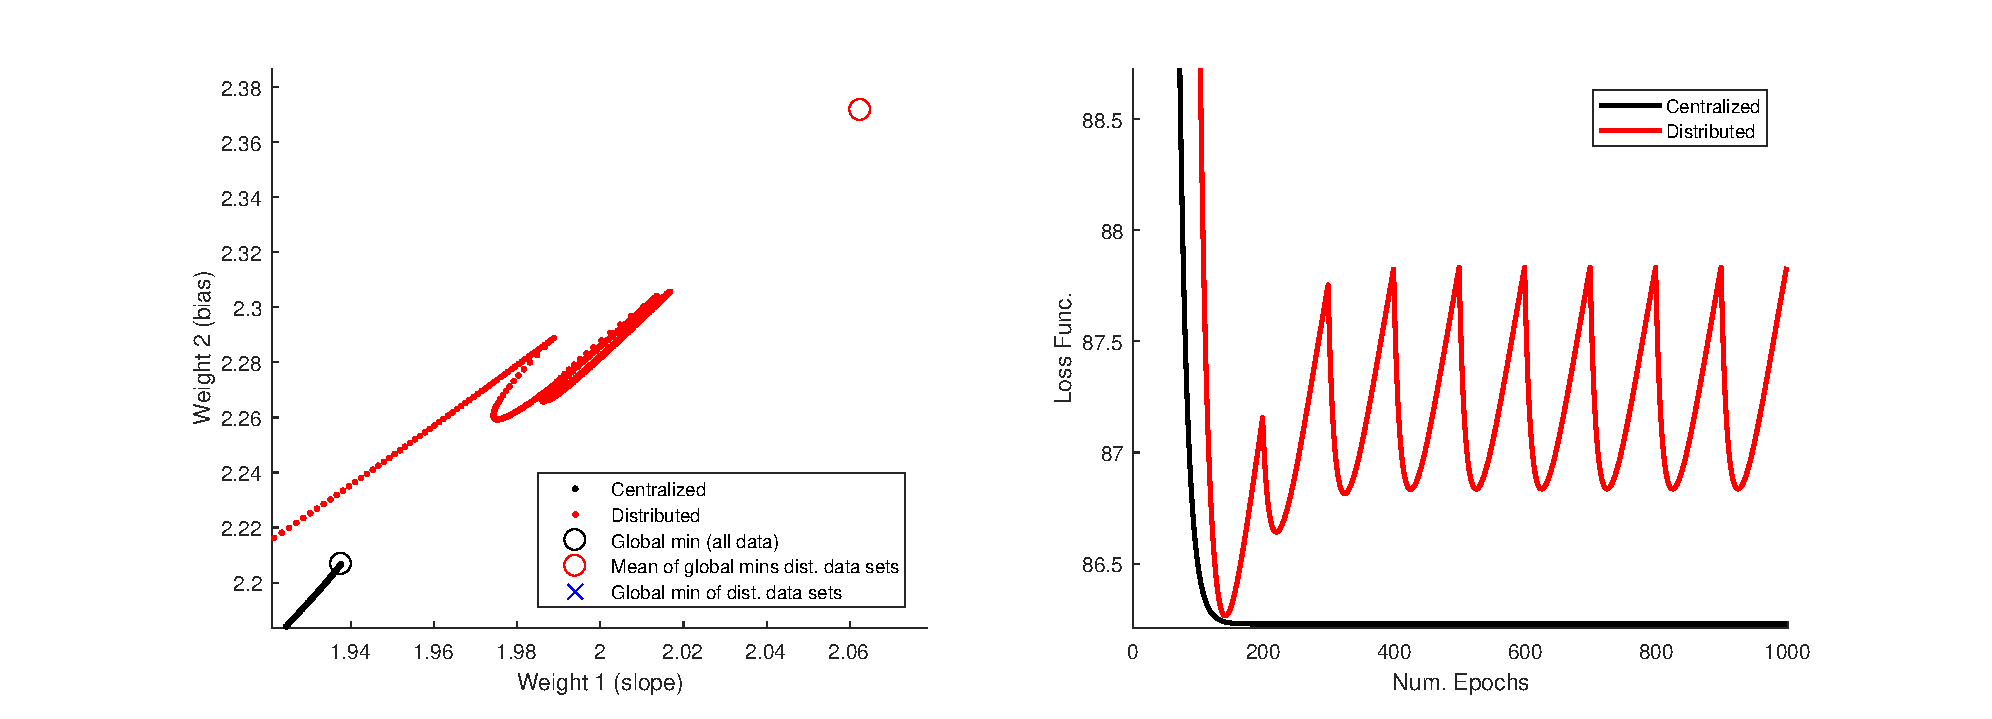
\includegraphics[width=20cm]{tau=100_zoom.eps}
\caption{Zoomed image: $\tau=100$}
\end{center}\end{figure}

   For both $\tau=10$ and $\tau=100$, it is clear that the distributed computing gets stuck in oscillations and training is not beneficial past a certain point. From this limited amount of experimentation, it also seems there is a trend between the loss function and $\tau$. As $\tau$ increases, the converges of the distributed system becomes farther from $\boldsymbol{w}^*$. Of course, this also depends on how close $\boldsymbol{w}^*$ is to $\bar{\boldsymbol{w}}^*$. In some cases, they can be close, although not shown here.

   \item \tbf{Dynamic $\tau$}

   One of the important results of this project is understanding the effect of $\tau$ on distributed learning. An important observation is that while, in general, $\boldsymbol{w}^*\neq\bar{\boldsymbol{w}}^*$, the points are close and the training at first performs similarly whether global updates are performed or not. Then as the training becomes more precise, global updates become more relevant to move towards $\boldsymbol{w}^*$. In the following, for the first time, we introduce the concept of ``dynamic $\tau$" such that global updates occur more frequently as the learning progresses.

   More specifically, at first $\tau = 100$, then every $200$ updates, either local or global, $\tau$ is reduced by half. The results are shown in the following figures.

      \begin{figure}[H]
\begin{center}
\advance\leftskip-3cm
\advance\rightskip-3cm
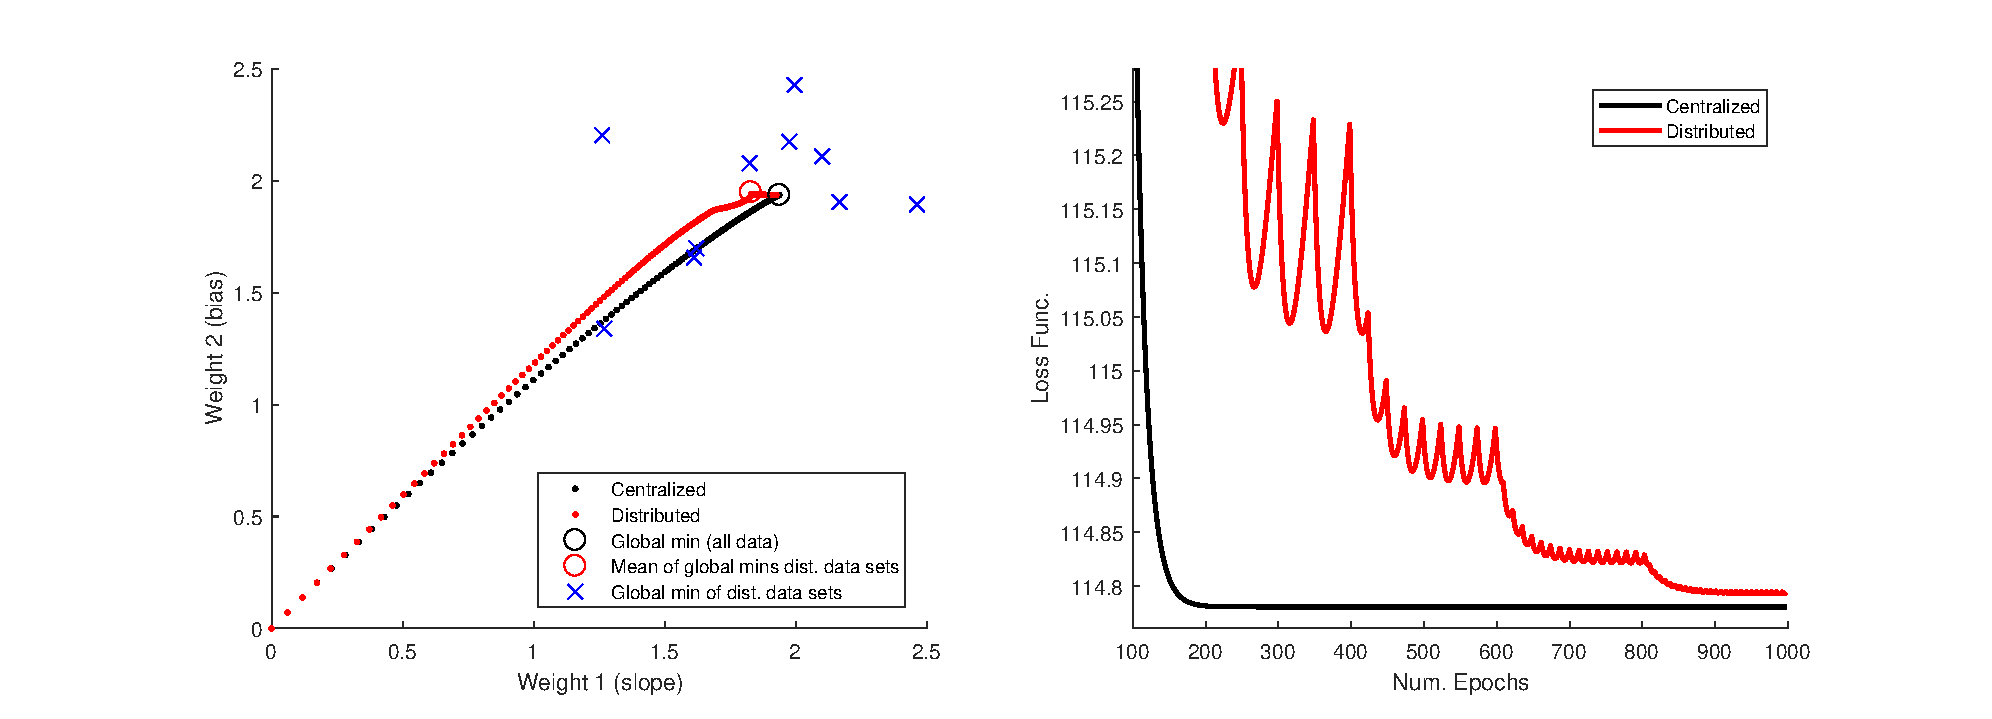
\includegraphics[width=20cm]{dynamic_tau.eps}
\caption{Dynamic $\tau$}
\end{center}\end{figure}

   \begin{figure}[H]
\begin{center}
\advance\leftskip-3cm
\advance\rightskip-3cm
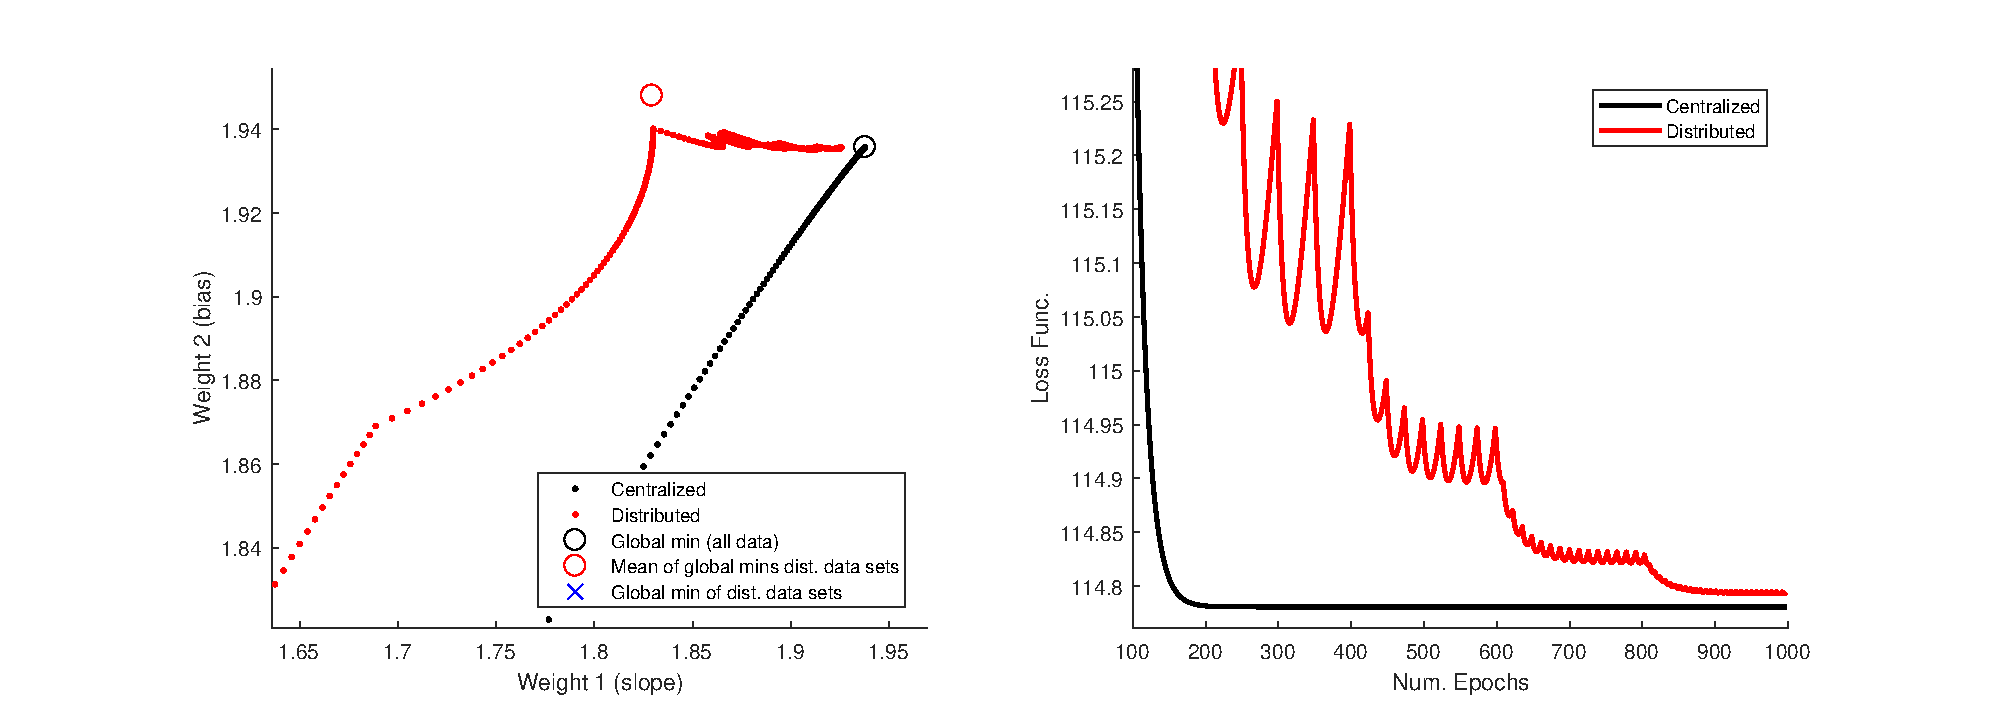
\includegraphics[width=20cm]{dynamic_tau_zoom.eps}
\caption{Zoomed image: Dynamic $\tau$}
\end{center}\end{figure}

   At first, the distributed training is moving towards $\bar{\boldsymbol{w}}^*$, then as $\tau$ is reduced the training moves toward $\boldsymbol{w}^*$. In the future, it may interesting to try other methods for adjusting tau, such as letting the system decide if it is converging or oscillating with training, and reducing $\tau$ when this occurs.

   \item \tbf{Data Shuffling in Distributed Linear Regression}

   We explore the effects of data shuffling on convergence speed and accuracy. To start, we consider an extreme case of data shuffling, where the data available to each node is random after $\alpha$ updates, either local or global. The motivation here is that this will be more reflective of stochastic gradient descent (SGD).

         \begin{figure}[H]
\begin{center}
\advance\leftskip-3cm
\advance\rightskip-3cm
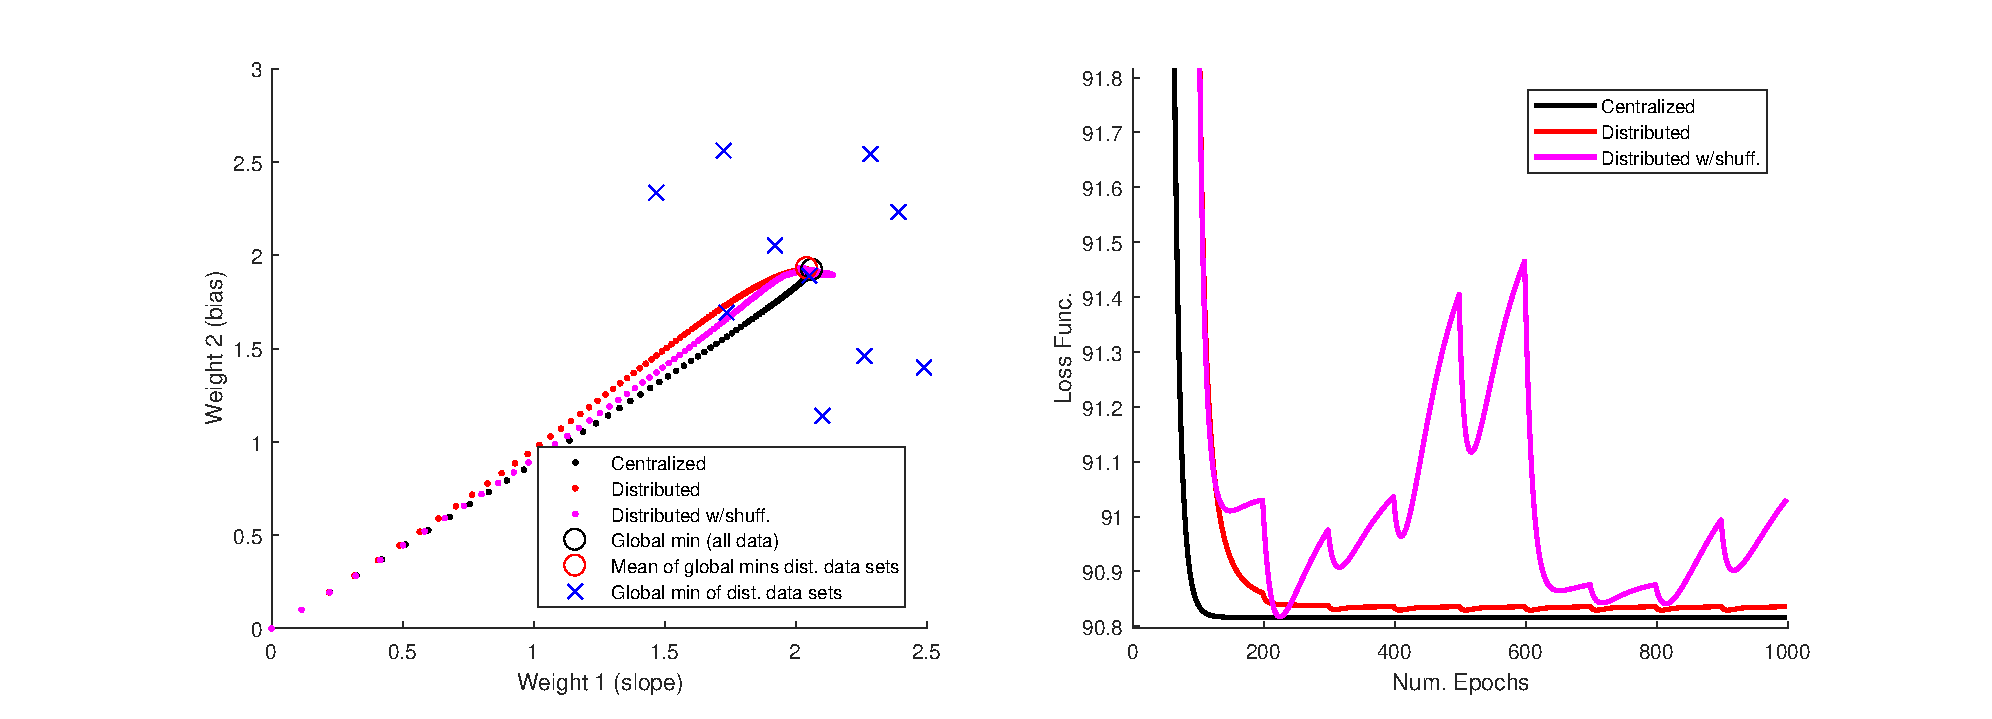
\includegraphics[width=20cm]{shuff_extreme.eps}
\caption{Comparison of distributed learning with and without shuffling, $\tau=100$, $\alpha=200$}
\end{center}\end{figure}

   \begin{figure}[H]
\begin{center}
\advance\leftskip-3cm
\advance\rightskip-3cm
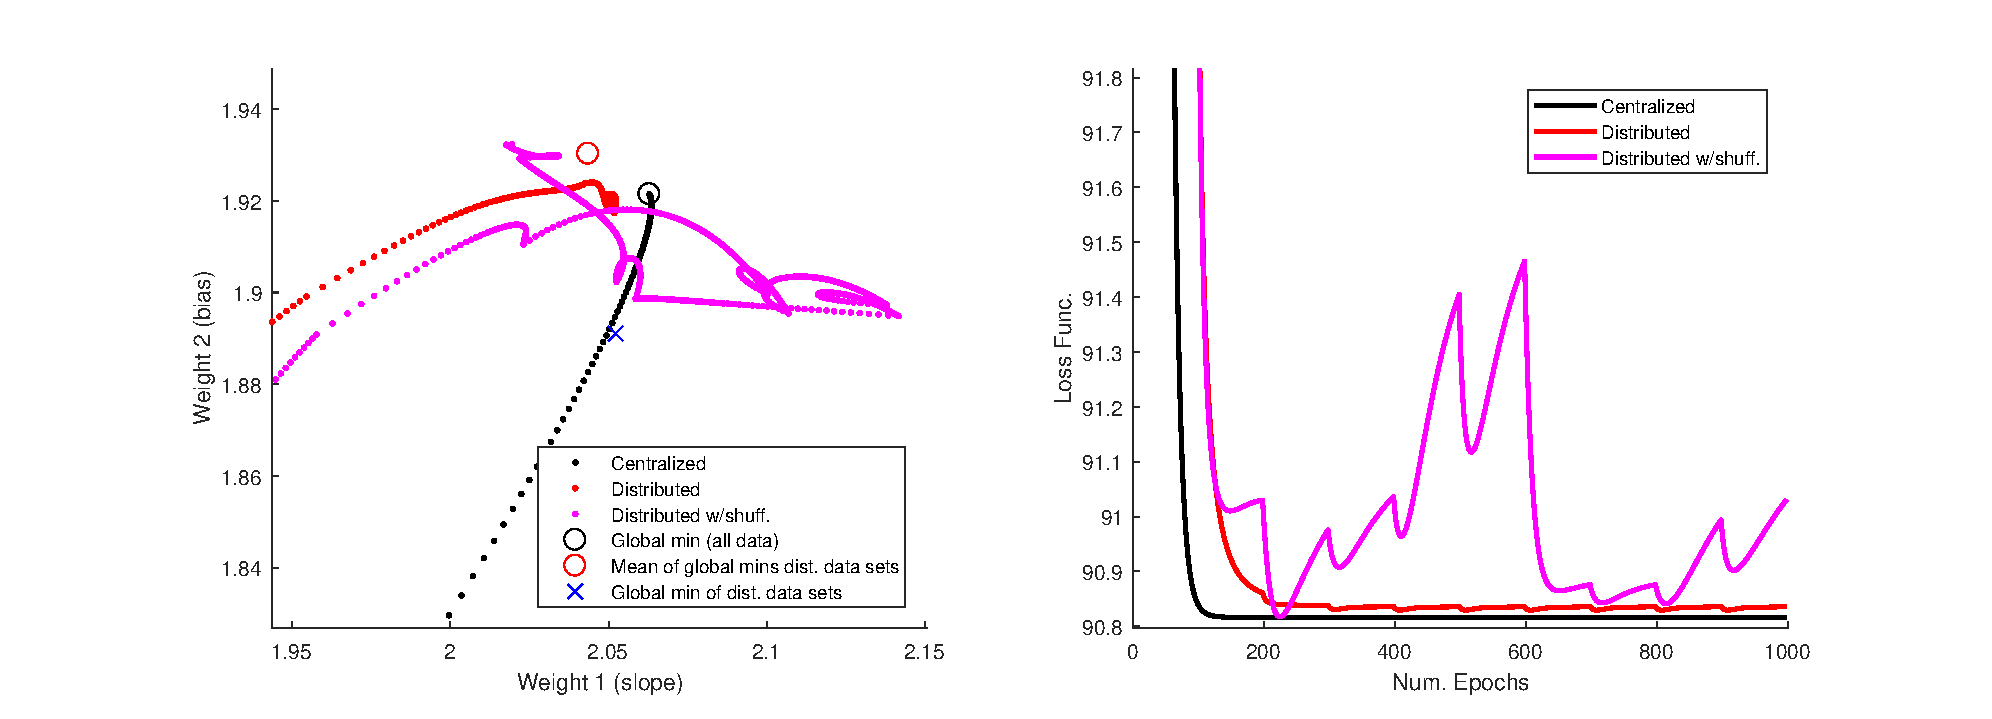
\includegraphics[width=20cm]{shuff_extreme_zoom.eps}
\caption{Zoomed image: Comparison of distributed learning with and without shuffling, $\tau=100$, $\alpha=200$}
\end{center}\end{figure}

   We find that in general, completing shuffling the data throughout training does not help convergence. With each new distribution of the data, the shuffled method starts converging to different points (i.e. $\bar{\boldsymbol{w}}^*$ is constantly changing for the shuffled training). As a result, the weights stop converging at a certain point and start sporadically jumping between different values around $\boldsymbol{w}^*$. Ultimately, there appear to be two issues with this version of shuffling. The first is that as the training progresses shuffling does not appear to be helpful. The second is that the shuffling is not strategically performed such that information of the training at the different nodes are used to configure the shuffling.

   In the following, we introduce a new method of shuffling which aims to solve the issues from the previous method. First, the shuffling is only done at the beginning of the training. Next, by using the locally learned weights at the nodes, we develop a scheme to dictate the data shuffling. The scheme works by finding the pair of nodes with weights which are farthest apart, and those nodes exchange half their local data points. Then, we go to the next two nodes with the next largest distance in weights and do the same. We continue this process through all the nodes. For the shuffled data, essentially, we are trying to move $\bar{\boldsymbol{w}}^*$ (not shown, changes with each shuffle) towards $\boldsymbol{w}^*$. This makes the shuffling more effective for the weights to converge towards $\boldsymbol{w}^*$.

   More specifically, in the following, we show a simulation where only one data shuffle is performed after $200$ iterations. Also, we use the idea of dynamic $\tau$ from the previous section to let the distributed systems converge to $\boldsymbol{w}^*$. By observing the loss function, in this scenario shuffling appears to improve the convergence rate.


            \begin{figure}[H]
\begin{center}
\advance\leftskip-3cm
\advance\rightskip-3cm
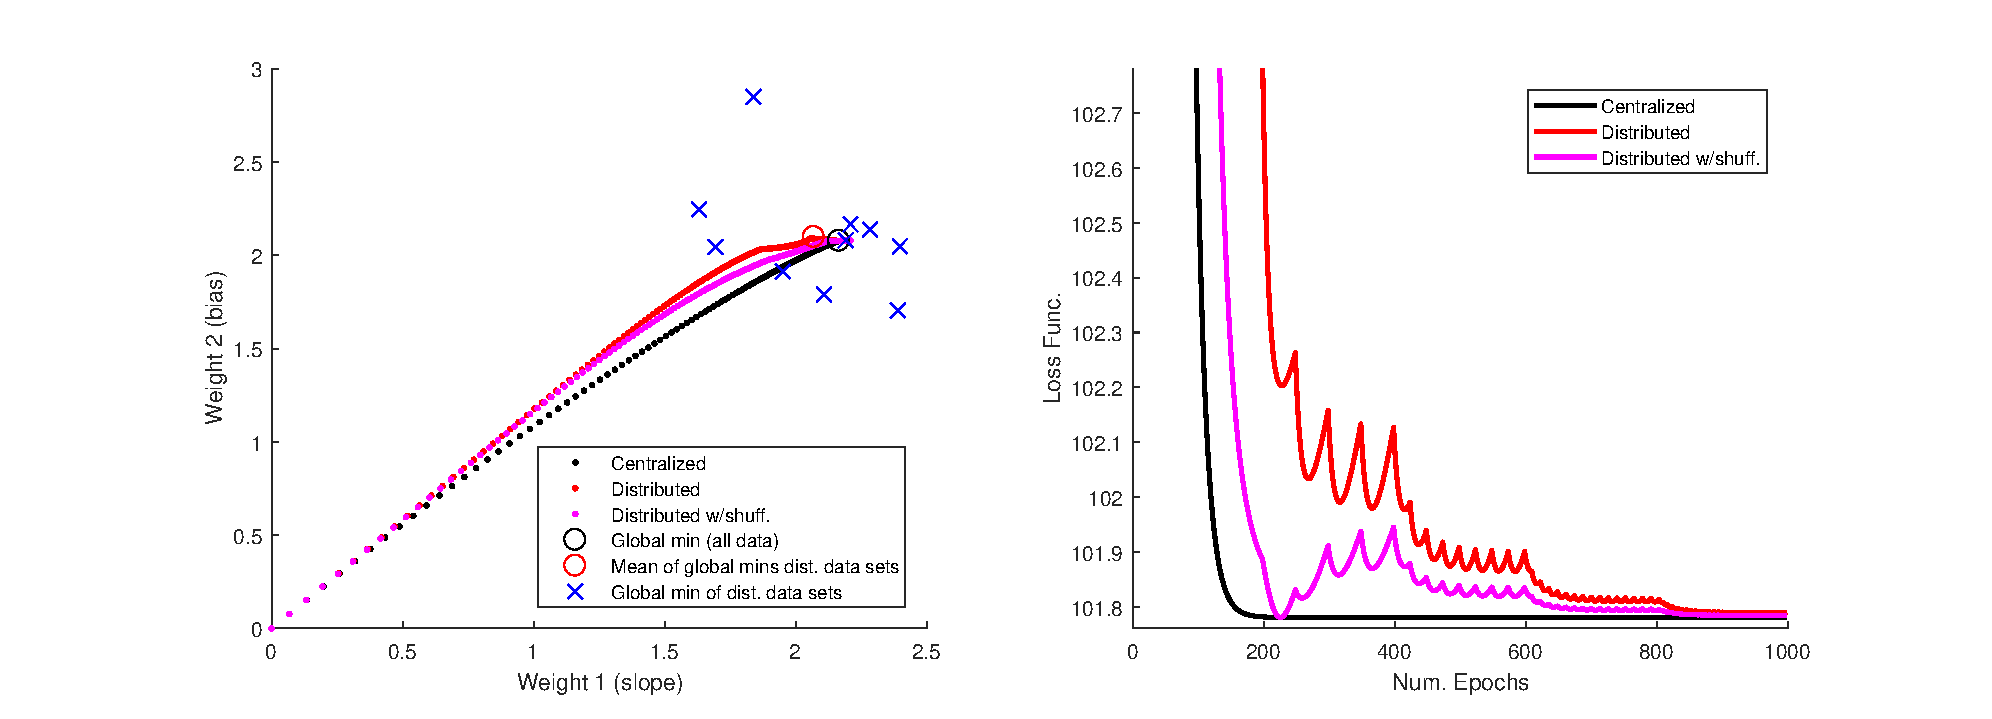
\includegraphics[width=20cm]{shuff2.eps}
\caption{Comparison of distributed learning with and without shuffling, dynamic $\tau$, with one shuffle after $200$ iterations}
\end{center}\end{figure}

   \begin{figure}[H]
\begin{center}
\advance\leftskip-3cm
\advance\rightskip-3cm
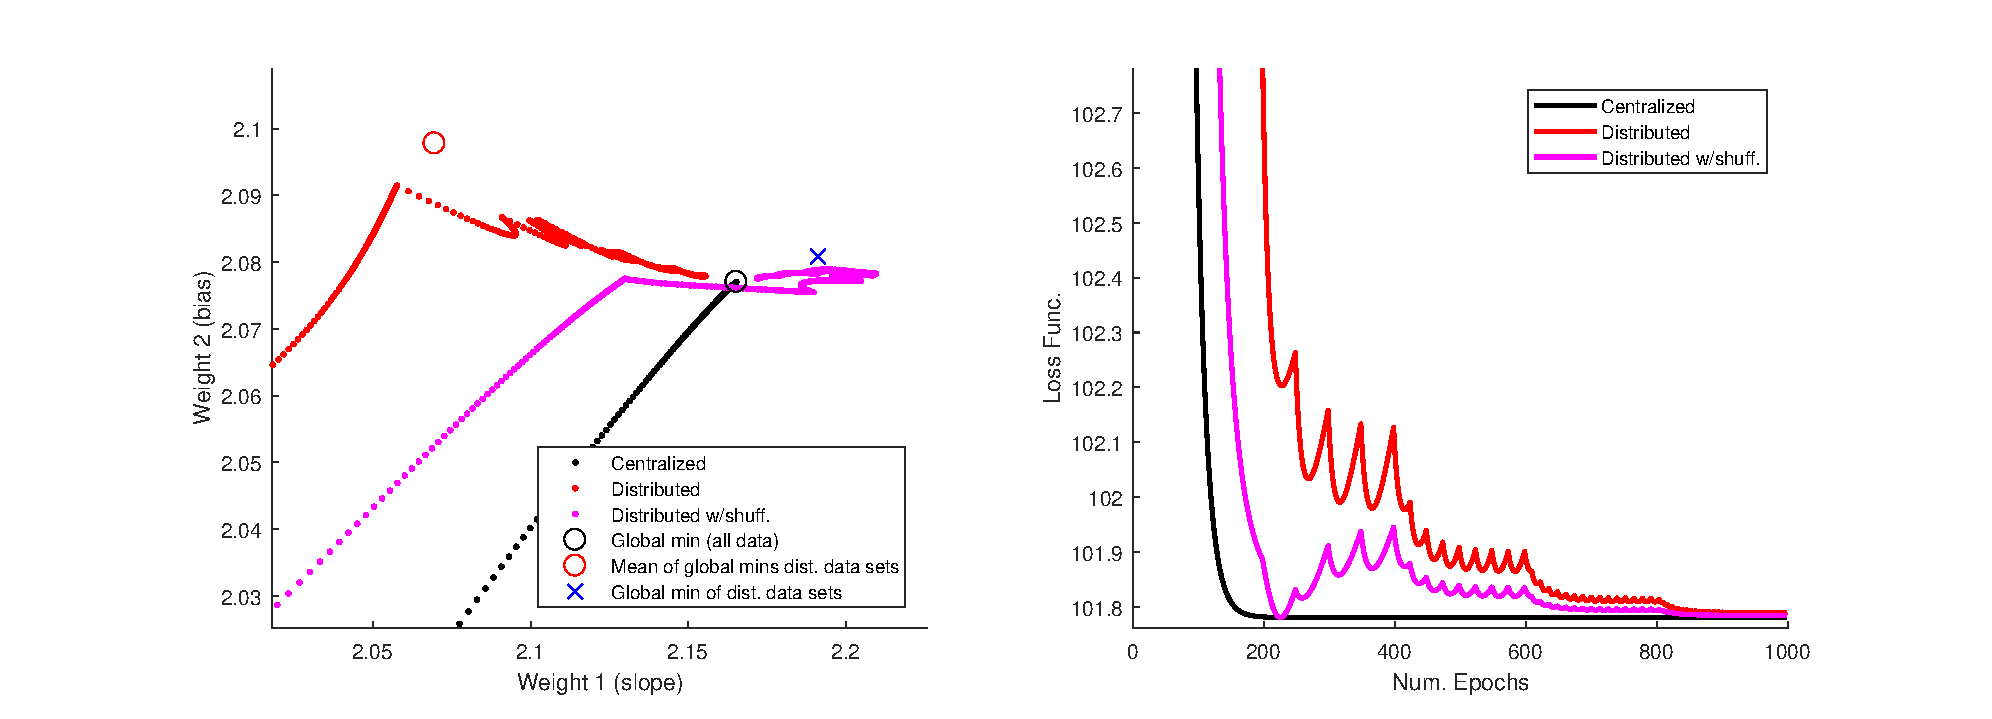
\includegraphics[width=20cm]{shuff2_zoom.eps}
\caption{Zoomed image: Comparison of distributed learning with and without shuffling, dynamic $\tau$, with one shuffle after $200$ iterations}
\end{center}\end{figure}

\end{enumerate}

\item \tbf{Future Directions}

In this work, the concept of distributed learning was investigated and many interesting research directions arise. For all of the simulations performed here, it would be useful to develop more concrete and general theory to explain what the findings are. Further simulations could also prove useful as the work performed here only looked at the results of single training runs, as opposed to doing many training simulations and observe the average performance. From this work, we have shown that in some cases shuffling does improve convergence and other times it does. It would be beneficial to investigate shuffling further with a larger variety of shuffling schemes, data and machine learning schemes. This may be able to provide a more definitive answer as to when shuffling benefits distributed learning.







\begin{thebibliography}{1}
\bibitem{ref1}Zinkevich, Martin, et al. "Parallelized stochastic gradient descent." Advances in neural information processing systems. 2010.
\bibitem{ref2}Lian, Xiangru, et al. "Can decentralized algorithms outperform centralized algorithms? a case study for decentralized parallel stochastic gradient descent." Advances in Neural Information Processing Systems. 2017.
\bibitem{ref3}Konečný, Jakub, et al. "Federated learning: Strategies for improving communication efficiency." arXiv preprint arXiv:1610.05492 (2016).
\bibitem{ref4}Wang, Shiqiang et al. "When edge meets learning: Adaptive control for resource-constrained distributed machine learning." IEEE INFOCOM 2018-IEEE Conference on Computer Communications. 2018
\end{thebibliography}
\end{enumerate}


\end{document}

